\chapter{Irodalom}
\pagestyle{headings}

Ezen fejezetben diplomamunkám elméleti háttereként szolgáló szakirodalmi hivatkozásokat foglalnám össze. Először a pásztázó mérőcsúcs mikroszkópia történetéről és működéséről írnék. A második alfejezetben a galvanikus korrózióra, a harmadikban pedig a mikroelektródokra, különös tekintettel a referenciaelektródokra térnék ki.

\section{Pásztázó mérőcsúcs mikroszkópia}

\subsection{Története}

A mikroszkópos technikák kezdetleges kialakulása a 16. században kezdte meg forradalmát, mikor elkészítették az első mikroszkópot. Fejlődésük és kialakulásuk szorosan összefügg az orvostudomány előrehaladásával, hiszen a sejtek tanulmányozását szabad szemmel nem tudták megtenni. Az idő múlásával párhuzamosan jelentek meg az eltérő típusú mikroszkóp családok: a fénymikroszkóp, elektronmikroszkóp és ennek egy alfaja, a pásztázó elektronmikroszkóp. Ez utóbbi csoportra térnék ki részletesebben dolgozatomban. [1]
A hagyományos mikroszkópiától alapvetően eltérnek ezek a módszerek. Fénymikroszkóp esetében a teljes látómezőről egyidejűleg kapunk adatokat, az összes mérési ponthoz tartozik egy érzékelő, mint például a CCD mátrixban az egyes fényérzékeny MOS kondenzátorok. Viszont együttes tulajdonságuknak mondható a pásztázó mikroszkópoknak, hogy egy szenzor van csak. A szenzort pozícionáljuk a vizsgálni kívánt minta feletti pontrendszer minden egyes pontjához, sorban, egymás után. A pontrendszer minden egyes pontján megállítjuk a szenzort és egy lokális mérést végzünk. A mérés eredményét eltároljuk a mérés koordinátáival együtt. A kapott adathalmazból egy képet tudunk készíteni ábrázolva a mérések eredményét a koordináták függvényében. A technika nagyon sokoldalú, hiszen kicserélve a mérőcsúcsot vagy a detektálás elvét rendkívül változatos méréseket végezhetünk el. A következő néhány bekezdésben röviden kitérek néhány mérföldkőnek számító technikára, különös tekintettel a dolgozatom szempontjából fontosabbakra. 
A pásztázó mérőcsúcs mikroszkópia (Scanning Probe Microscopy, SPM) története az irodalom szerint a pásztázó alagút mikroszkóp (Scanning Tunnelling Micsocopy, STM) kifejlesztésével kezdődött 1981-ben az IBM svájci laboratóriumában dolgozó Gerd Binning és Heinrich Rohrer munkájának köszönhetően \cite{binnig1982tunneling}. A technika lényege az alagúthatás, melyet a minta és a rendkívül hegyes mérőcsúcs között létesített nagy feszültség létrehozásával érnek el. A minta és a mérőcsúcs közötti távolság éppen úgy van megválasztva, hogy az elektronok számára pusztán energiájuk alapján egy áttörhetetlen potenciálgátat jelentsen. Az alagúthatás jelenségének köszönhetően azonban ezt a potenciálgátat át tudják törni egy bizonyos távolságon belül. A távolságot a mérés során úgy változtatja egy automatikus visszacsatolási kör, hogy ez éppen bekövetkezhessen. A mérőcsúcs tehát pontosan követi a minta topográfiáját. Mivel ez a mérés során folyamatosan ismert, ebből és az X-Y koordinátákból a minta magasságtérképe kirajzolható rendkívül nagy pontossággal. A technikával akár egyedi atomokat is láthatunk. A technika olyan nagy jelentőségűnek bizonyult, hogy már 1986-ban Nobel díjat adományoztak a két kutatónak.
Az atomerő mikroszkópia (Atomic Force Microscopy, AFM) elveit, ugyanebben az időben, szintén Binning találta fel, majd néhány évre rá sikeresen kivitelezték a technikát a gyakorlatban is először \cite{binnig1986atomic}. Az STM-hez hasonlóan ez a mikroszkópia is piezomotorokat használ a nagy felbontású képalkotás miatt, de ez a módszer határozottan szofisztikusabb működésű az előzőnél. Szigetelő és vezető tulajdonságú felületek esetén is atomi szintű felbontást nyújt. Egy lézernyaláb visszaverődéses érzékelési elvén alapul. A mérőcsúcs egy mikroméretű tartókaron helyezkedik el, ami elhajlik a mintán és a mérőcsúcson lévő atomok kölcsönhatása végett. A tartókar elhajlását egy kísérő lézer érzékeli, ami szintén a tartókaron található, és ez egy fotodiódasorra visszaveri a ráirányított sugarat. Tehát a mérőcsúcs bizonyos mértékben el fog hajlani, a mintán fellelhető topográfiai elváltozások következtében, emiatt pedig a visszaverődési szöge meg fog változni a lézernyalábnak. Az egyes pozícióknál mért magasságra a lézernyaláb beesési szögéből tudunk következtetni. A tartókaron lévő lézernyaláb mozgatása nagyon kicsi erőt igényel, így akár egységnyi atomok közti kölcsönhatásokat is nyomon tudjuk követni. Érzékenysége sok újfajta alkalmazásnak nyitott teret, mint például szigetelő és vezető anyagok atomi szintű vizsgálata. [4]
Megjegyezném azonban, hogy a dolgozatomban is alkalmazott pásztázó referencia elektród technikát (Scanning Reference Electrode Technique, SRET) már 1979-ben kifejlesztette és sikerrel alkalmazta Hugh Isaacs [5]. Az említett kutató főleg korrózióval foglalkozott, és a SRET-et egy korróziós probléma megoldására fejlesztette ki. A mérés során egy mikroméretű referenciaelektródot mozgatunk, amivel a lokális korrózió során a fém felületén valós időben mérhetjük a potenciált, a folyamat megzavarása nélkül. Ez tehát egy nem invazív elektrokámiai módszernek. Helyi korrózió esetében, potenciál mezők keletkeznek az elektrolitban, mivel a katódos oldal felszíne felé elektromos áram folyik az anódos területről. A technika azonosítja ezen területeket és a valós idejű, akár a rendkívül kis potenciálú, változásokat detektálja az aktív minta felületén. Hasznos eszköznek bizonyult az in situ korróziós vizsgálatoknál, mint például fémbevonatok delaminációja és különböző ötvözetek, fémek korróziós viselkedésének vizsgálatához. [6,7]
A pásztázó vibráló elektród technikát (Scanning Vibrating Electrode Technique, SVET) már 1974-ben használták az extracellurális áramerősségek mérésére. [8] Majd az 1980-as években kezdte Hugh Isaacs a különböző korróziós folyamatok vizsgálatához továbbfejleszteni és alkalmazni. [9] Működése során az oldatban méri a minta felett a helyi áramerősség sűrűségének eloszlását, és ezzel feltérképezi a felületen lezajló elektrokémiai folyamatokat in situ, miközben kialakulnak. Mivel a mért áramerősség függ a reakció sebességétől, a technika kvantitatív. Mérőcsúcsként a mintára merőlegesen rezgő mikroméretű platina pálcát használ, amivel az elektromos potenciált mérjük a rezgőmozgás két szélsőhelyzetében egy ún. „lock-in” erősítő segítségével. A technika szorosan összefügg a SRET-el, tulajdonképpen ez annak egy továbbfejlesztett változata. 
Korábbiakban említve, a SRET technika előnyének mondható a SVET-el szemben, hogy noninvazív technika és a korróziós vizsgálatokban a folyamatok megzavarása nélkül térképezhetjük fel az anódos és katódos oldalait a céltárgynak. Illetve az elektrolit oldatot se keveri olyan mértékben a vizsgálat során. Ennek ellenére, a SVET mégis érzékenyebb technika, ami a vibráló mérőcsúcsnak és az emiatt javuló jel-zaj viszony arányának köszönhető. SRET-el az elektrokémiai folyamatban kialakuló potenciál különbségeket mérjük a minta felett az elektrolit oldatban, míg SVET-el az áramerősség sűrűséget vizsgálva ad információt és alkot képet az oldatban lezajló elektrokémiai folyamatokról.Elektroanalitikai szempontból az 1980-as években mérföldkövet jelentett, mikor Allen J. Bard és csoportja lefektették az elméleti és gyakorlati alapjait a pásztázó elektrokémiai mikroszkópiának (Scanning Electrochemical Microscopy, SECM). [10,11] Megjegyzendő azonban, hogy három évvel korábban Engstrom már végzett hasonló méréseket. [12] Egy mikroelektróddal pásztázott egy másik elektródot, melyek eltérő potenciáljait bipotenciosztáttal irányította. Így generáló-gyűjtő módban alkalmazhatta az elektródokat és a mikroméretű mérőcsúcshoz diffundált a másik elektród által generált anyag. Mikromanipulátort használt a mozgatásához. Általánosságban véve a módszer lényege, hogy egy mikroelektródot alkalmazunk mérőcsúcsként, melynél a hegyen is elektrokémiai reakció játszódik le, és ezzel pásztázzuk a vizsgálandó mintánkat. A mikroelektród a mérés során polarizálva van egy potenciosztát segítségével, tehát a mérőcsúcs tulajdonképpen egy amperometriás mérőkör munkaelektródja. 
Korábban említett közleményekből idézve, megemlítenék még egy ismert jelenséget, ami jelentős a felületek vizsgálata során, ez pedig a visszacsatolás (feedback) jelensége. Ezen belül is megkülönböztetünk pozitív és negatív visszacsatolást. Ha a mérőcsúcsunkat közelítjük a céltárgyunkhoz, és ez a távolság eléri merőlegesen, a minta felületétől számítva, a 3d-nél kisebb értéket, (d alatt az elektród aktív felületének átmérőjét értjük) folyamatosan csökken vagy nő a mért áramerősség. 
Pozitív visszacsatolás esetén, minél közelebb jutunk a vezető felülethez, annál nagyobb áramerősséget detektál a műszerünk a tömbfázisban mérthez képest. Ezt amperometriás méréseknél tapasztalhatjuk, vezető felületekhez közelítve a mérőelektródot. Magyarázata, hogy a vezető felület és a mérőcsúcs között kialakult pozitív visszacsatolási kör egyre rövidebbé válik, ahogy közeledünk a minta felületéhez. Vagyis reverzibilis reakció esetén, visszaoxidálódik eredeti formájába a mérőelektród által redukált anyag. 
Negatív visszacsatolás esetén az áramerősségben folyamatos csökkenést detektálunk, ahogy a mérőcsúcs közelebb ér a felszínhez. Ezt szigetelő tulajdonságú felszínek vizsgálata során figyelhetjük meg, aminek oka, hogy a mérőelektród aktív felületénél nullára csökken az oxidálható anyag koncentrációja. A csökkenő távolság megakadályozza, hogy átalakítható anyag diffúzió révén pótolható legyen. Emiatt a detektált áramerősség is nullára csökken, vele arányosan.
 3d távolság felett ezeket az összefüggéseket az áramerősségben és a mért távolságban nem tapasztaljuk. Ilyenkor egy steady state állapot alakul ki, ugyanannyi anyag oxidálódik, mint amennyi redukálódik.
Eredetileg amperometriás detektálásokra lett kifejlesztve a technika, de nagy hátránya ennek, hogy kevés kémiai információt ad. Nem sokkal később viszont megjelent a potenciometriás változata, Nagy Géza és Benjamin Horrocks kutatásainak köszönhetően, melyben a hidrogénion aktivitást térképezték. [13] Lehetővé vált tehát a tényleges kémiai környezet feltérképezésére is a megfelelő ionszelektív mikroelektród alkalmazásával. Manapság egyre elterjedtebben használják a technikát, mivel kiválóan alkalmazható különböző ionok szelektív térképezésére megfelelő ionszelektív mérőcsúcs alkalmazásával. [14] Ez pedig a korróziós vizsgálatok során rendkívül előnyös tulajdonság. [15] A technika kifejlesztésekor már rendelkezésre állt makroméretű ionszelektív elektródok egész sora, többek között egy magyar kutatócsoportnak köszönhetően, Pungor Ernő vezetésével. [16]

\subsection{Működése}

A SPM alapja, a többi mikroszkópiás technikához hasonlóan, a raszteres képalkotás. A mérőcsúcsot, ami jelen esetben egy mikroelektród, mozgatjuk egy előre meghatározott algoritmus szerint, a vizsgálandó minta felett. A mikroelektród egy mikromanipulátorhoz van rögzítve, amit egy számítógépes programmal egyszerűen kezelhetünk. Általában meanderező mozgást követ a szoftver, de lehet például vonalpásztázást és összetett vonalpásztázást is alkalmazni algoritmusként. [17] A mérések előtt kell megadnunk a paramétereket a programnak (mozgás, lépésköz és ennek ideje, intervallum).  megkülönböztetünk amperometriás és potenciometriás méréseket. Amperimetriás mód esetén a cella egy mérőelektródból, egy referencia elektródból és egy segédelektródból áll. A mérőelektródot mozgatjuk, míg a referencia- és segédelektród a pásztázási területtől odébb helyezkedik el, hogy ne zavarja a mérést. Potenciometriás módban pedig egy referencia elektródból és egy ionszelektív elektródból épül fel a cella, és az ionszelektív elektród potenciálját mérjük a referencia elektródunkhoz képest.


\begin{figure}
\centering
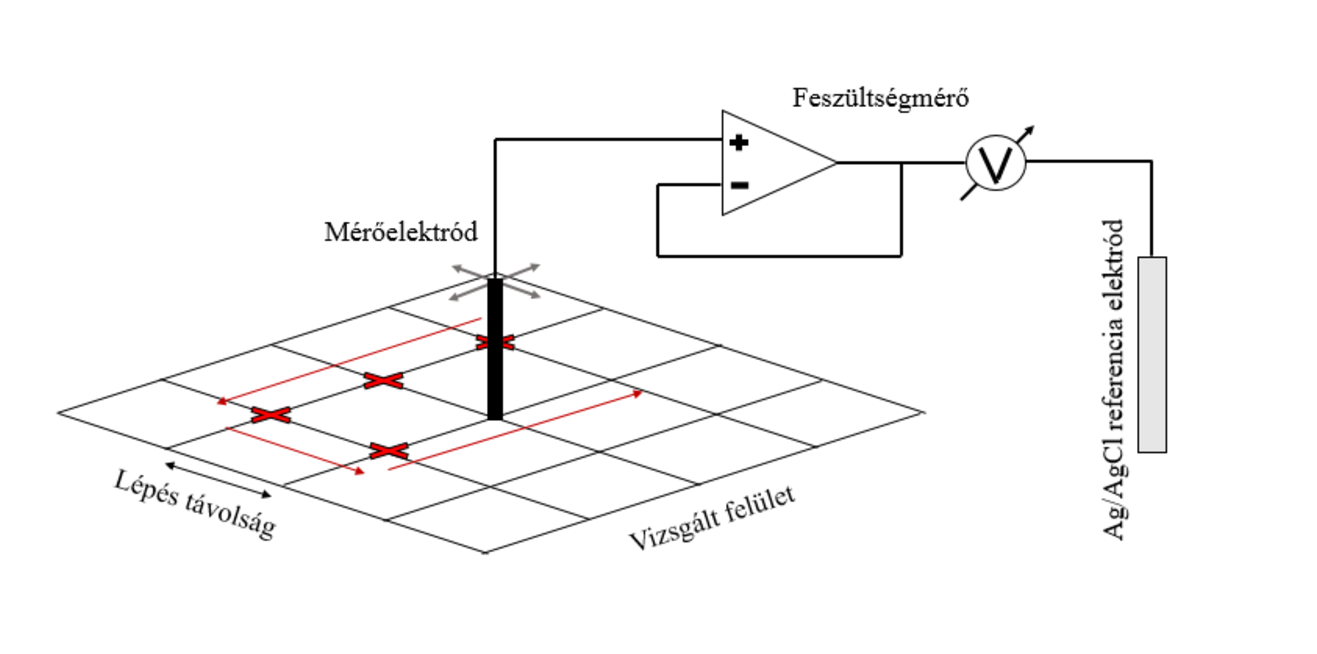
\includegraphics[width=0.8\textwidth]{img/spm.eps}
\caption{Pásztázó elektrokémiai mikroszkóp működésének szemléltetése.}
\label{fig:PEKM}
\end{figure}

\begin{figure}
\centering
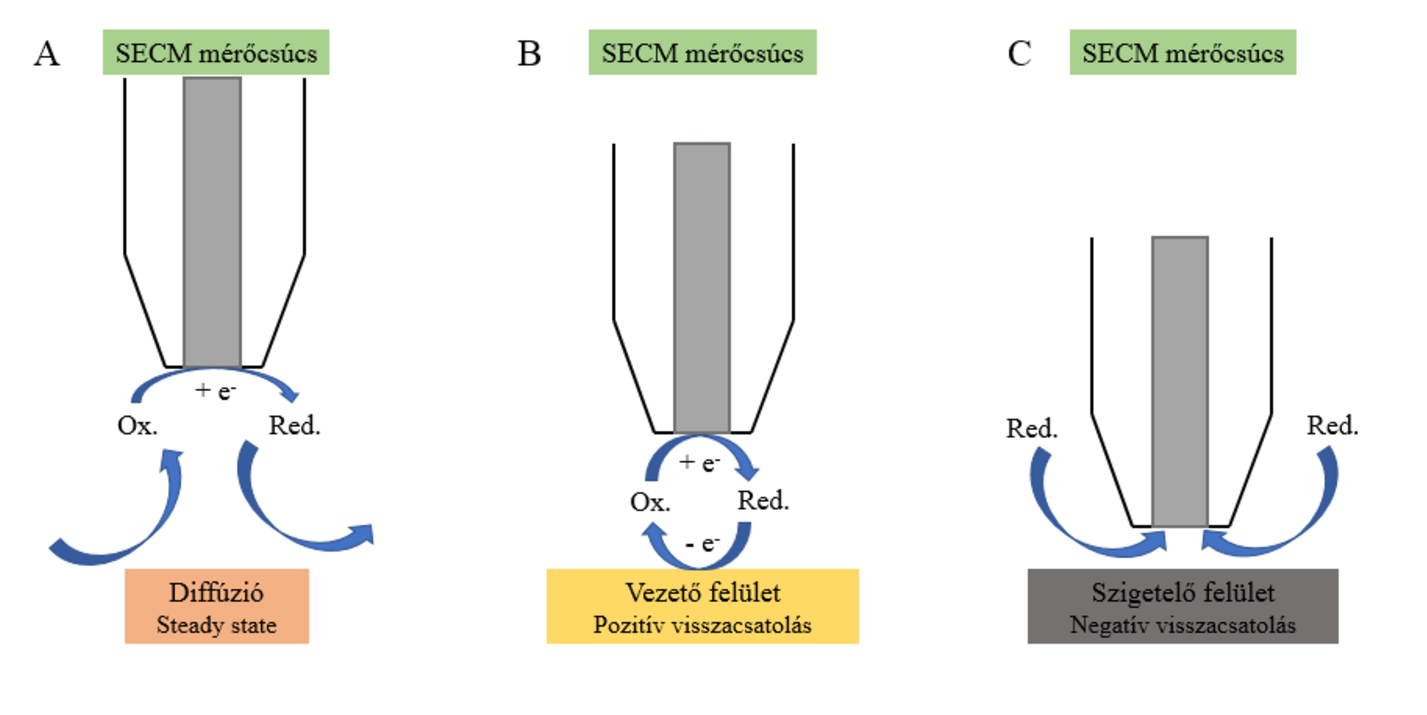
\includegraphics[width=0.8\textwidth]{img/feedback.eps}
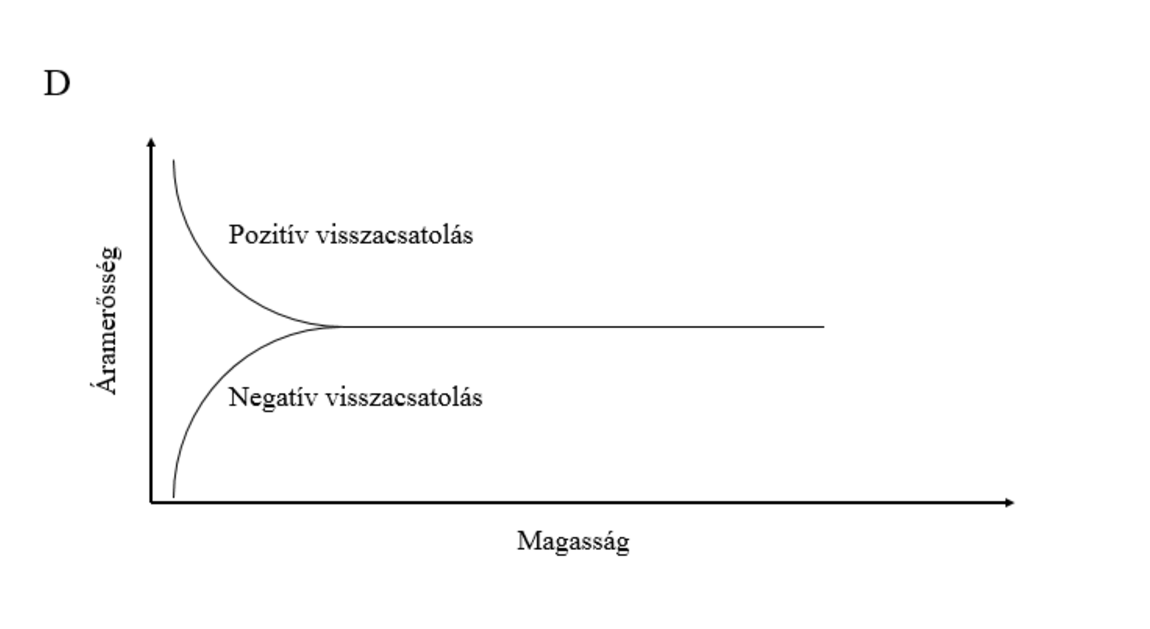
\includegraphics[width=0.8\textwidth]{img/feedback2.eps}
\caption{Visszacsatolás jelensége:
A: 3d magasság felett steady state állapot, ugyanannyi oxidáció, mint redukció
B: vezető felület felett pozitív
C: szigetelő felett negatív visszacsatolás
D: áramerősség a magasság függvényében. A magasság a mérőcsúcs vége és a céltárgy felszíne közti távolságra értendő}
\label{fig:feedback}
\end{figure}
